\clearpage
\begin{landscape}
	\begin{figure}[htbp]
	\centering
		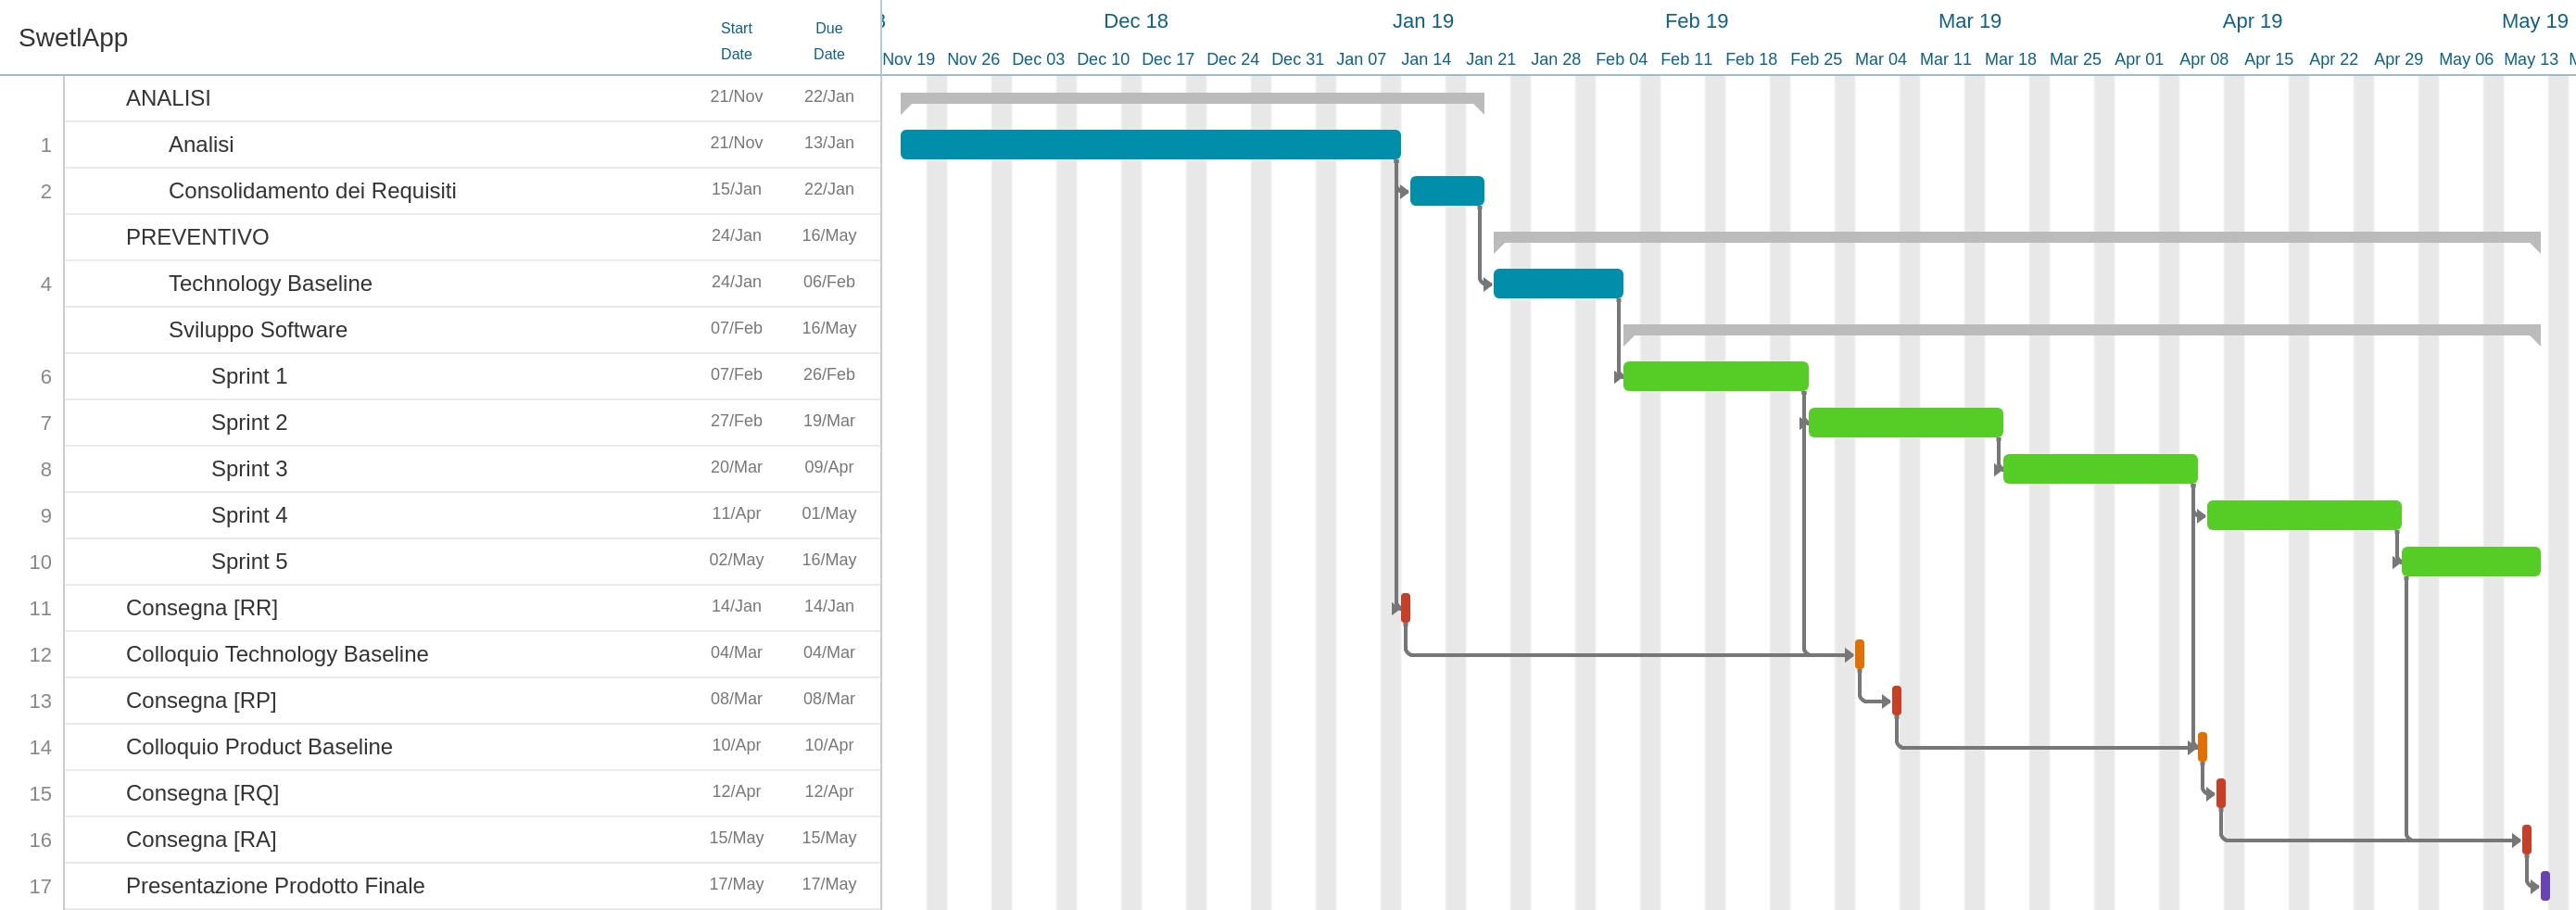
\includegraphics[width=\linewidth ,keepaspectratio]{../includes/pics/grafici/Swetlapp.jpeg}
		\caption{\label{fig:gantt-swetlapp}diagramma di Gantt ad alto livello dell'intero progetto}
	\end{figure}
\end{landscape}
\clearpage
\section{Pianificazione}
\label{sec:pianificazione}
La pianificazione elaborata dal gruppo \emph{duckware}, è stata costruita cercando di adattare il modello di sviluppo agile alle scadenze temporali riportate in \hyperlink{scadenze}{§1.5}. Ne risulta una suddivisione in due macro periodi: 
\begin{itemize}
	\item \textbf{Investimento};
	\item \textbf{Preventivo}.
\end{itemize}
Questi periodi sono stati poi suddivisi in fasi, pianificate come indicato in Figura \ref{fig:gantt-swetlapp}. 
Ciascuna di queste fasi è stata ulteriormente scomposta in sotto-attività, da svolgere durante la fase stessa per facilitarne il completamento. In seguito, verrà illustrata una rappresentazione finale ad alto livello del lavoro che verrà svolto per tutte le fasi di ogni macro periodo:
\subsection{Investimento}
\label{sec:investimento}
\subsubsection{Analisi}
Il periodo di analisi ha inizio il 20-11-2018 con la formazione e conoscenza del gruppo, e si conclude il 14-01-2019 in coincidenza con la consegna dei documenti per l'entrata in progetto. Durante questo lasso di tempo le attività da svolgere riguarderanno esclusivamente la documentazione:
	\begin{itemize}
		\item \textbf{Norme di Progetto}: in questa attività vengono elaborate le \emph{Norme di Progetto}, un documento redatto dall'Amministratore in cui sono elencate e stabilite le norme che il gruppo \emph{duckware} deve seguire durante tutta la durata del progetto. Questa fase è considerata molto importante in quanto il documento stabilisce anche le direttive e gli strumenti che verranno usati per la stesura dei documenti;
		\item \textbf{Studio di Fattibilità}: in questa attività gli Analisti compilano lo \emph{Studio di Fattibilità}, un documento contenente le analisi dei vari capitolati proposti durante la loro presentazione, essenziale per la scelta del capitolato che verrà poi svolto. Attività critica in quanto può bloccare l'inizio dell'\emph{Analisi dei Requisiti};
		\item \textbf{Analisi dei Requisiti}: in questa attività si prevede la stesura dell'\emph{Analisi dei Requisiti} da parte degli Analisti. Tale documento racchiude lo studio e gli approfondimenti del capitolato scelto ed è considerata un'attività importante e critica per la continuazione del progetto;
		\item \textbf{Piano di Progetto}: in questa attività il \markg{Responsabile} analizza le attività necessarie e le loro scadenze per la buona riuscita del progetto mentre l'Amministratore analizza i rischi nei quali il gruppo \emph{duckware} può incombere durante lo sviluppo del progetto. Il documento \emph{Piano di Progetto} può risultare bloccante per la stesura della Lettera di Presentazione. \\Inoltre durante questa attività vengono suddivise le risorse disponibili;
		\item \textbf{Piano di Qualifica}: in questa attività gli Analisti individuano i metodi che garantiranno la qualità del prodotto, questi ultimi sono riportati nel documento \emph{Piano di Qualifica};
		\item \textbf{Glossario}: in questa attività viene scritto un \emph{Glossario}, cioè un documento dove vengono inseriti e descritti tutti i termini considerati ambigui;
		\item \textbf{Lettera di Presentazione}: in questa attività viene scritta una \emph{Lettera di Presentazione} formale, necessaria per presentare il gruppo \emph{duckware} come fornitore al committente.
	\end{itemize}
\begin{figure}[htbp]
	\centering
	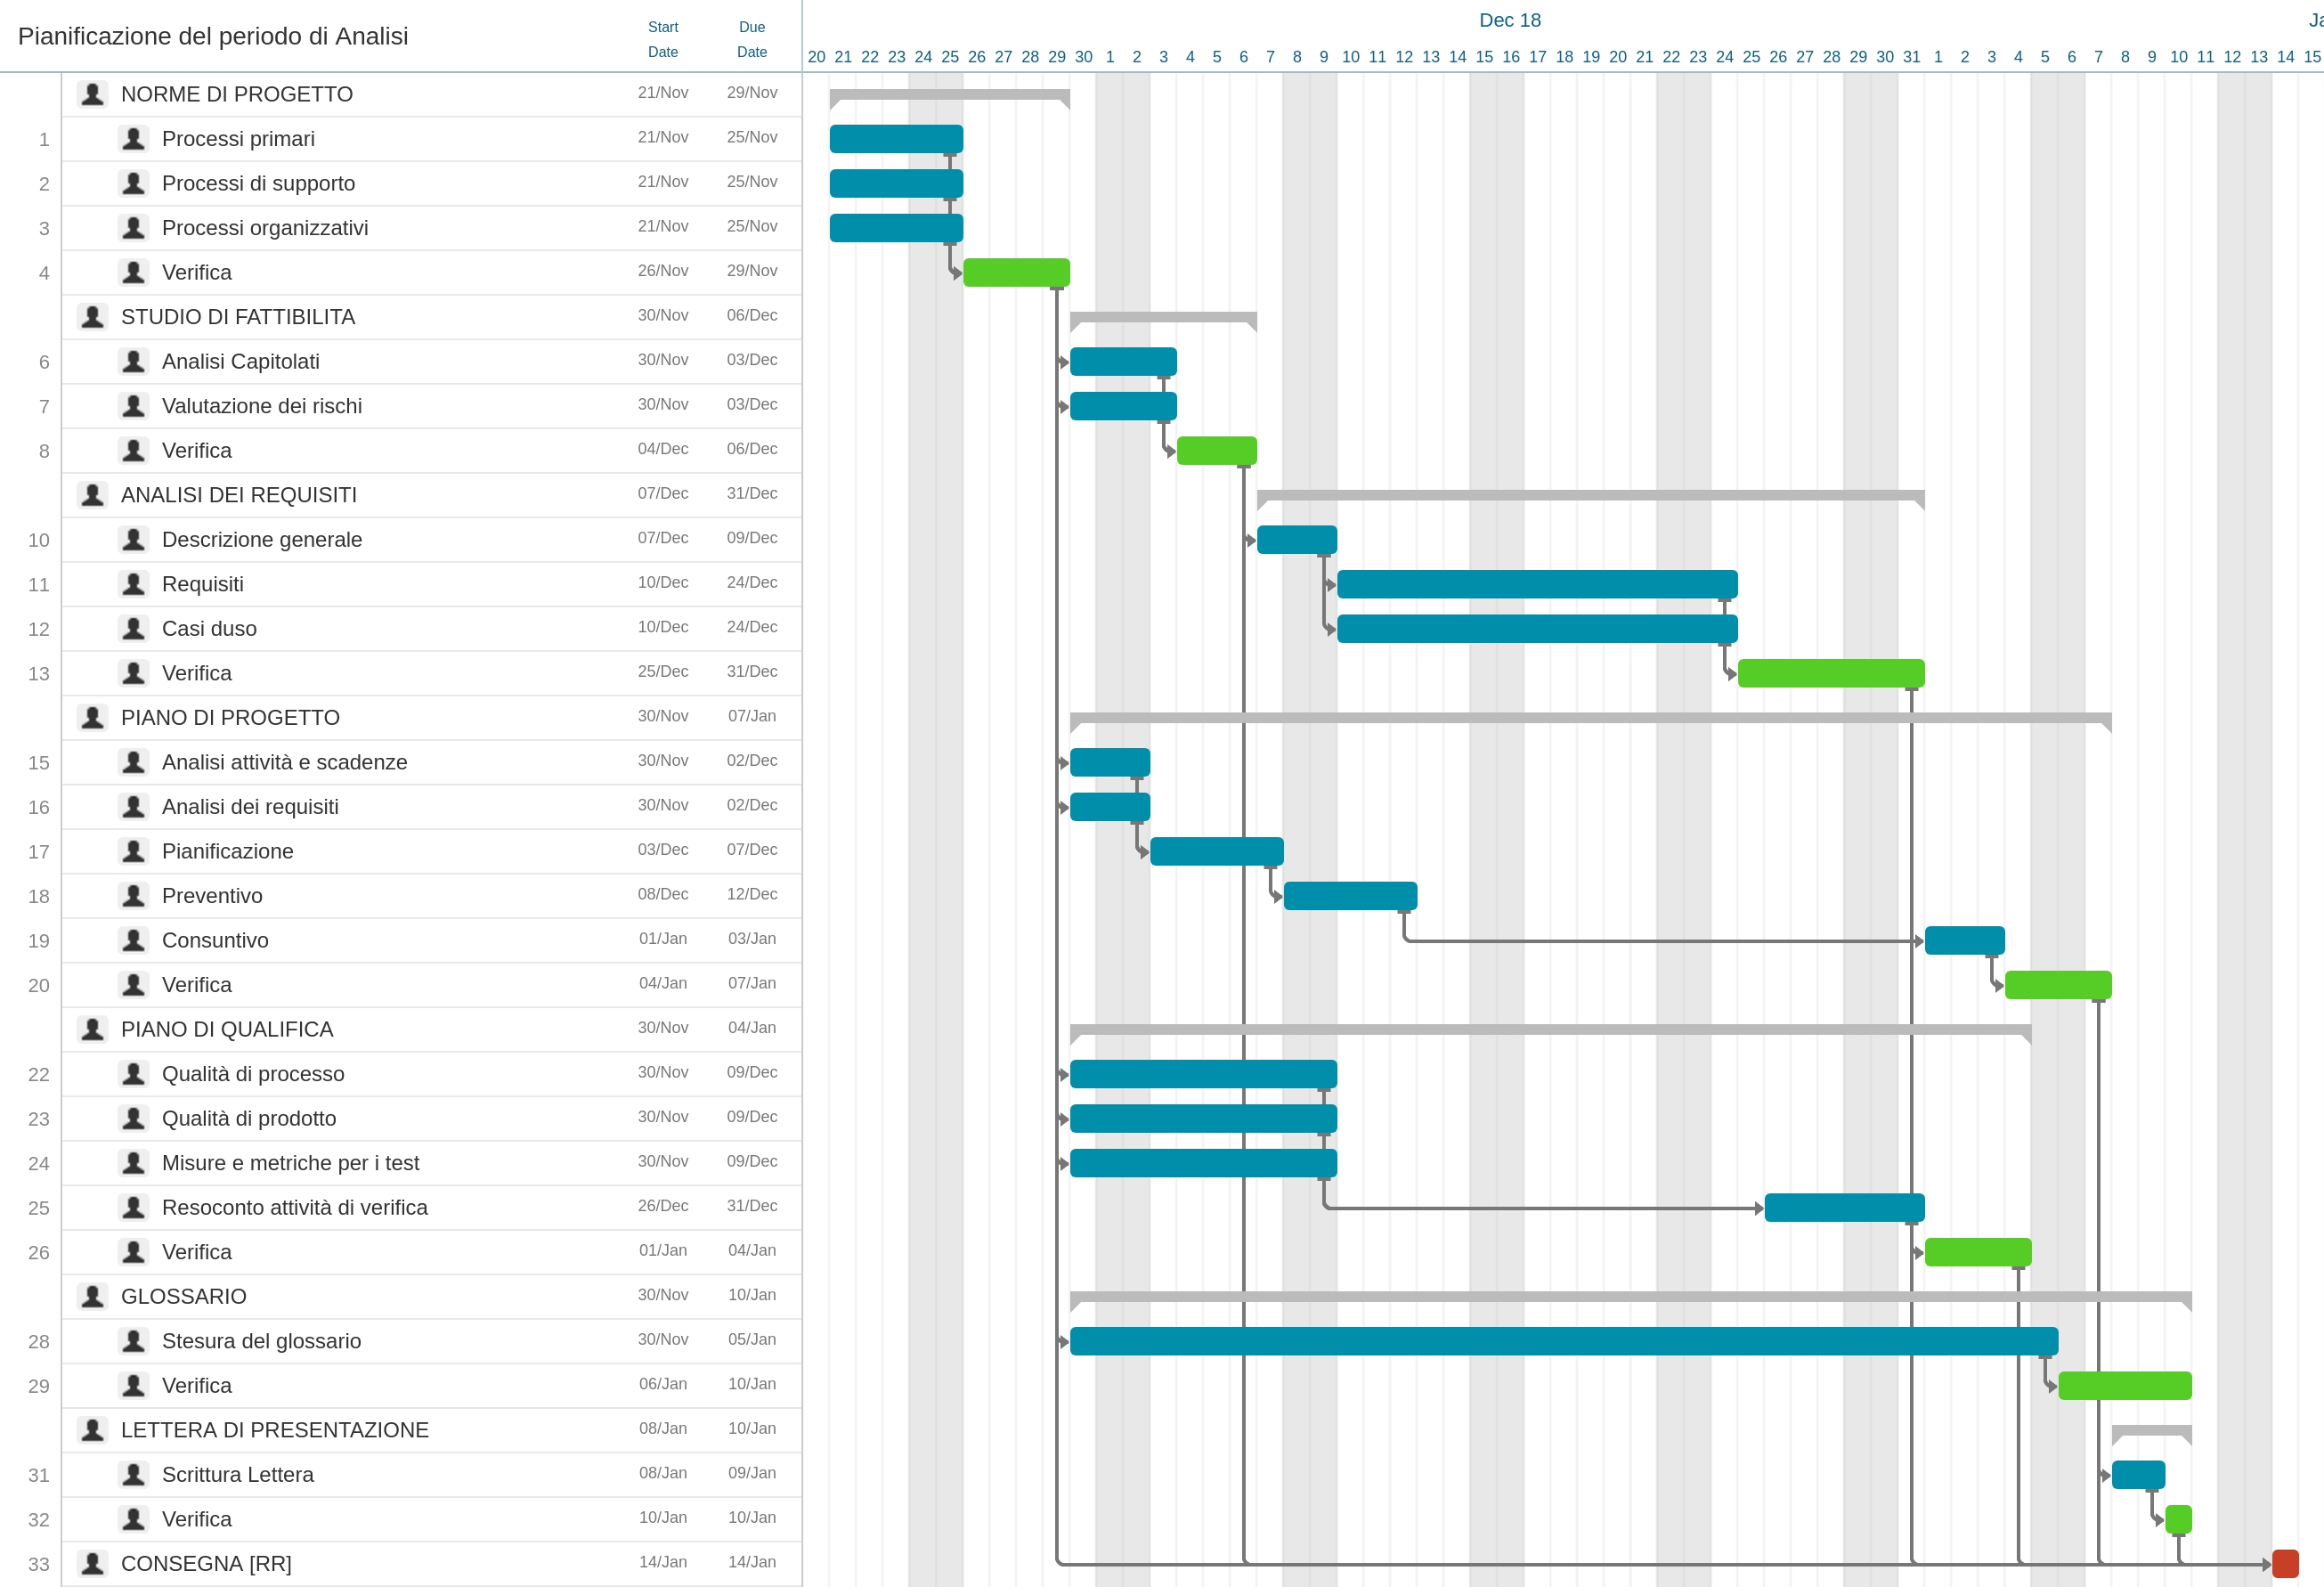
\includegraphics[width=15cm,keepaspectratio]{../includes/pics/grafici/Gantt_analisi.jpeg}
	\caption{\label{fig:gantt-analisi}diagramma di Gantt del periodo di Analisi}
\end{figure}

\clearpage
\subsubsection{Consolidamento dei requisiti}
La fase di consolidamento dei requisti ha inizio il 14-01-2019 con la consegna dei documenti per la prima scadenza e termina il 21-01-2019 con la presentazione della \emph{Revisione dei Requisiti}. Durante questo intervallo l'attività principale sarà il miglioramento dell'\emph{Analisi dei Requisiti} e dei documenti stilati in prospettiva dell'inizio del periodo di Progettazione della base applicativa richiesta.\\
\begin{figure}[htbp]
	\centering
	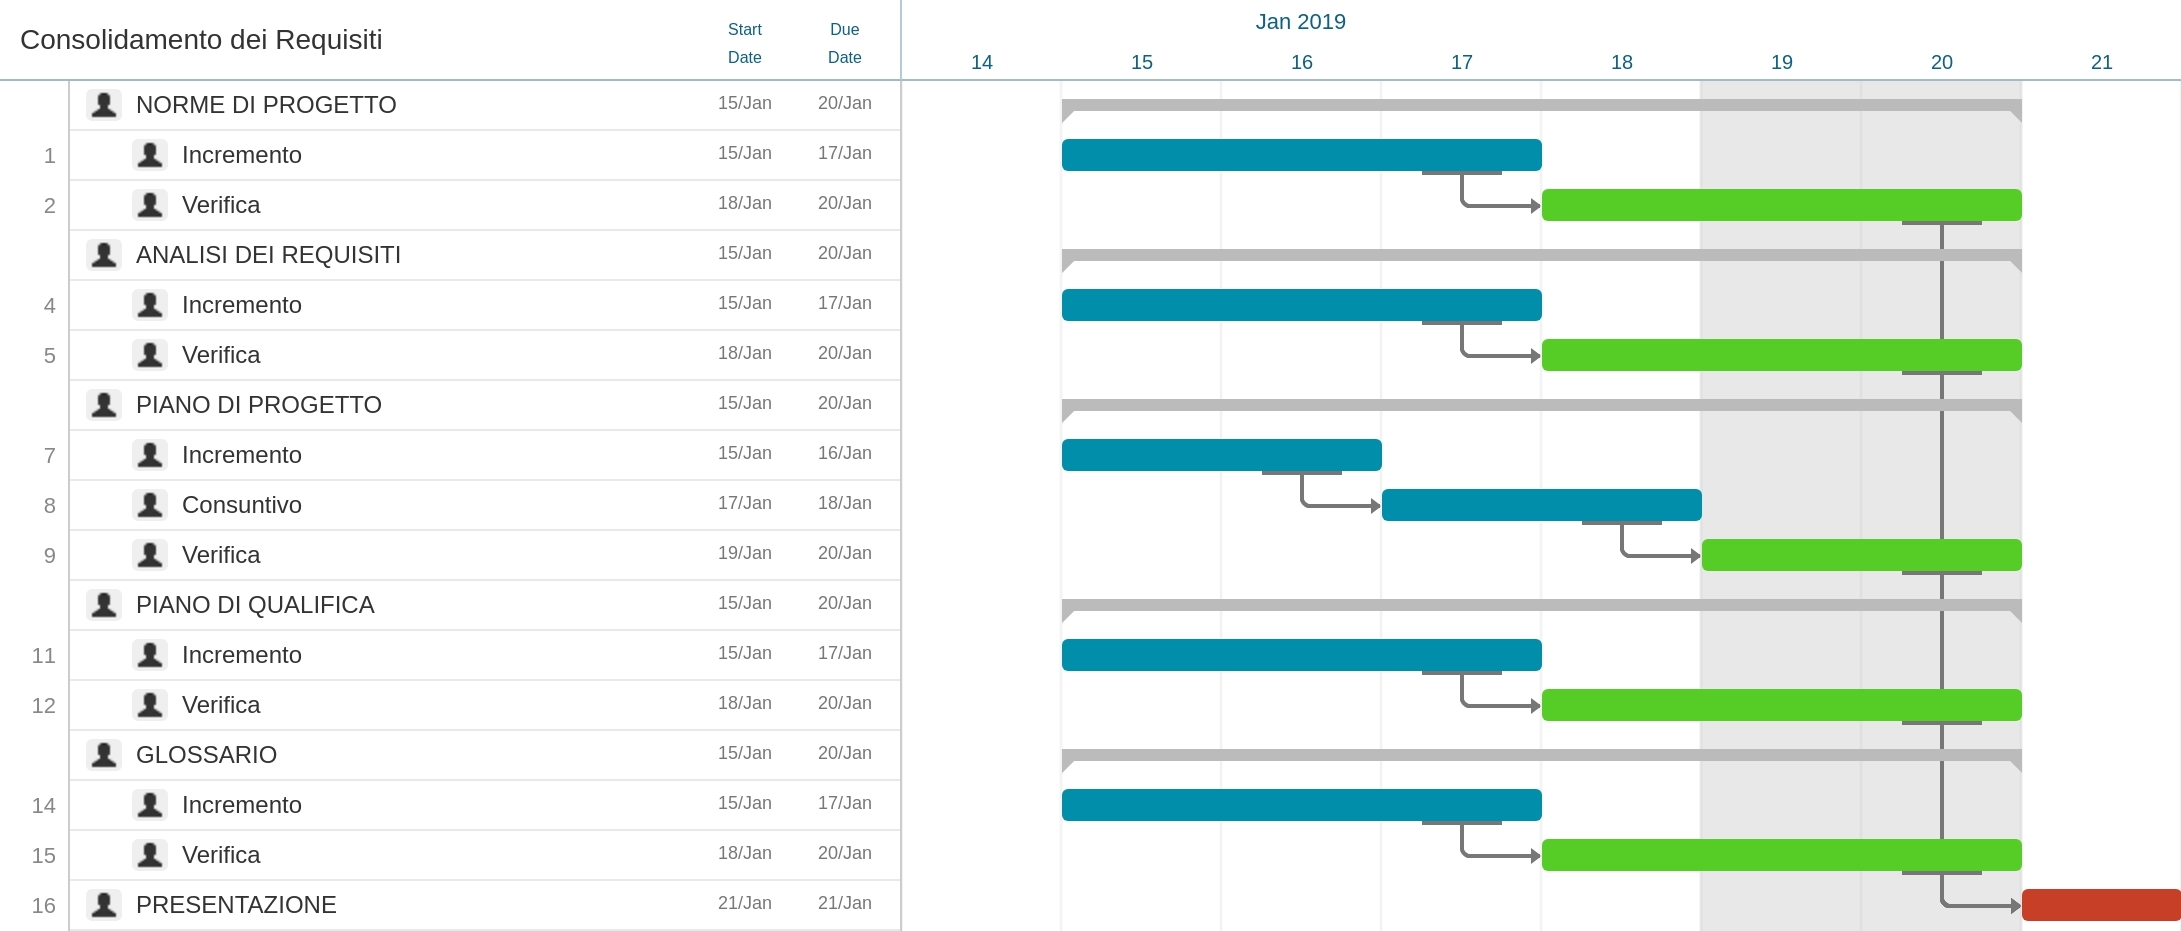
\includegraphics[width=15cm,keepaspectratio]{../includes/pics/grafici/Gantt_consolidamento_requisiti.jpeg}
	\caption{\label{fig:gantt-consolidamento}diagramma di Gantt per il Consolidamento dei requisiti}
\end{figure}

\clearpage
\subsection{Preventivo}
\label{sec:preventivo}

\subsubsection{Technology Baseline}
\label{sec:technology_baseline}
La prima fase che costituisce il periodo di Preventivo è la \emph{Technology Baseline} e si estende dal 22-01-2019, giorno successivo alla \emph{Revisione dei Requisiti}, al 06-02-2019, giorno in cui inizia lo \emph{Sviluppo software}. Essa ha lo scopo di definire l'architettura tecnologica del prodotto e comporta un'attenta analisi degli strumenti da utilizzare. 
\`E importante sottolineare che questa fase è stata volutamente separata dalla fase \emph{Sviluppo software} in quanto comprende anche un'attività di Apprendimento delle Tecnologie da parte di tutto il team \emph{duckware}. Normalmente, questa attività non è presente nella pianificazione, in quanto il team di sviluppo viene modellato in base alle competenze richieste dalla \emph{Technology Baseline}.
Le attività principali saranno:
	\begin{itemize}
	\item \textbf{Discussione del Feedback}: prima di effettuare altre attività, il gruppo deve analizzare e discutere gli esiti della consegna precedente, così da rivedere eventuali punti critici evidenziati e quindi apportare migliorie  specifiche al prodotto. Questa \markg{task} è utile anche per pianificare il lavoro da svolgere all'interno di questa fase;
	\item \textbf{Adeguamento al feedback, Incremento e Verifica}: in queste attività, vengono eseguite delle modifiche sui documenti \emph{Norme di Progetto}, \emph{Analisi dei Requisisti}, \emph{Piano di Progetto}, \emph{Glossario} e \emph{Piano di Qualifica} seguendo le indicazioni risultanti dalla Revisione dei Requisiti. \\ 	\`E fondamentale precisare che con "incremento" si intende un'aggiunta di valore al termine di un'iterazione sul prodotto stesso, comportando quindi dei cambiamenti talvolta sostanziali al prodotto, sia su base estetica che funzionale;
	\item \textbf{Backlog}: La creazione di un \markg{Backlog} è la base fondante del metodo Agile. Durante questa attività, infatti, si definiscono tutte le task da svolgere durante il corso del progetto, assegnando loro un grado di priorità proporzionale all'importanza del requisito sul quale operano;	
	\item \textbf{Technology Baseline}: durante questa attività, i progettisti hanno il compito di dare una definizione architetturale al prodotto, scegliendo le tecnologie, i \markg{framework} e le librerie da utilizzare durante la realizzazione del software. Come si evince, l'inadempimento di questa attività precluderà l'accesso allo sviluppo software;
	\item \textbf{Sprint Planning}: Questa attività, contestualmente alla Technology Baseline, consiste nel pianificare le task contenute nel backlog, assegnandole a un appropriato ciclo di sprint, basandosi sulla priorità conferita loro in fase di creazione del backlog. 
	\end{itemize}
\begin{figure}[htbp]
	\centering
	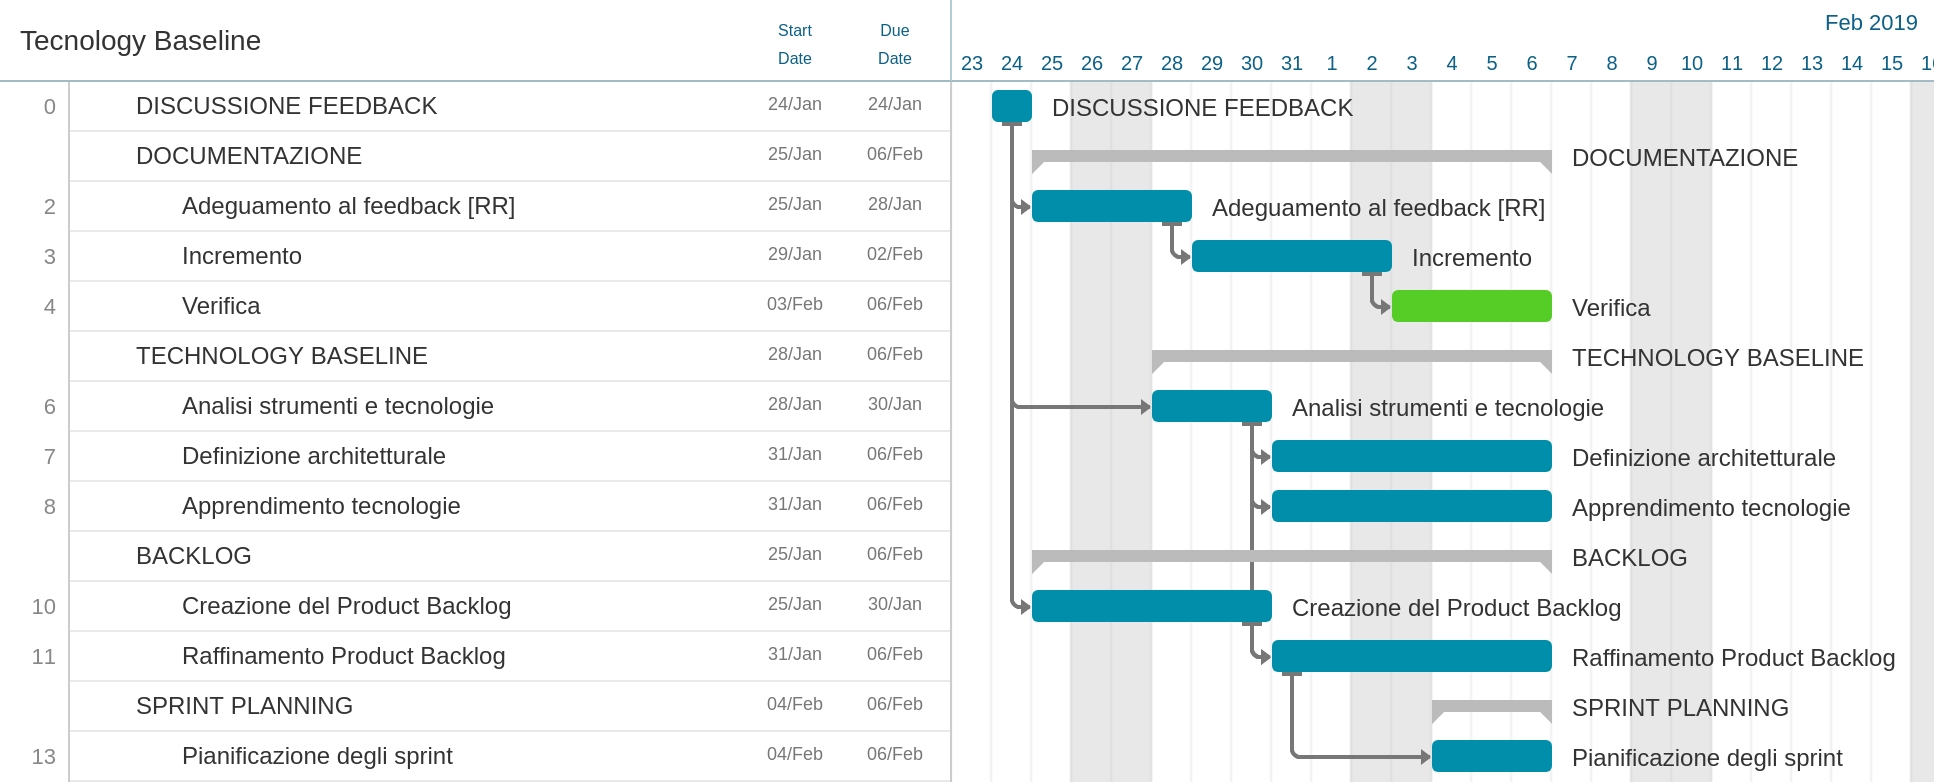
\includegraphics[ height=8cm, width=15cm]{../includes/pics/grafici/Technology_Baseline.jpeg}
	\caption{\label{fig:gantt-tb}diagramma di Gantt Progettazione architetturale}
\end{figure}

\clearpage
\subsubsection{Sprint 1}
Con lo \emph{Sprint 1}, che comincia il 07-02-2019 e si protrae fino al 26-02-2019, ha inizio il periodo di \emph{Sviluppo Software}. In questa fase si eseguono le attività assegnate durante la Technology Baseline:   
	\begin{itemize}
		\item \textbf{Sprint Planning}: si tratta di una riunione ad inizio sprint, nella quale il team si accorda sugli obiettivi da raggiungere entro fine sprint. Inoltre vengono identificati i requisiti necessari al completamento delle singole attività;
		\item \textbf{Adeguamento al feedback, Incremento e Verifica}: in queste attività, vengono eseguite delle modifiche sui documenti \emph{Norme di Progetto}, \emph{Analisi dei Requisisti}, \emph{Piano di Progetto}, \emph{Glossario} e \emph{Piano di Qualifica} seguendo le indicazioni risultanti dalla Revisione dei Requisiti. \\ 	\`E fondamentale precisare che con "incremento" si intende un'aggiunta di valore al termine di un'iterazione sul prodotto stesso, comportando quindi dei cambiamenti talvolta sostanziali al prodotto, sia su base estetica che funzionale;
		\item \textbf{Sviluppo Software}: questa \markg{task} consiste nel tradurre in codice quanto definito nell'attività \emph{"Technology Baseline"}. Essa comprenderà un periodo iniziale di configurazione degli ambienti di lavoro, un periodo di codifica ed infine una fase di testing e verifica. Questa attività risulta essere critica in quanto è fortemente vincolata da quanto esplicitato in \emph{Norme di Progetto} a livello qualitativo, e in \emph{Analisi dei Requisiti} a livello funzionale. \`E bene specificare che il risultato di questo sprint sarà il deployment di un \markg{Proof of Concept} dell'applicativo richiesto, il quale avrà lo scopo di dimostrare la fattibilità del prodotto, oltre a dare l'idea di quali saranno le sue caratteristiche funzionali principali.
		\item \textbf{Sprint Review}: si tratta di un meeting di fine sprint ed ha lo scopo di verificare quali funzionalità sono state implementate durante il corrente sprint;
		\item \textbf{Sprint Retrospective}: segue lo \emph{Sprint Review} ed è un incontro in cui il team di sviluppo discute su quanto è stato fatto durante lo sprint, sulle difficoltà avute durante lo sviluppo e sulle migliorie che si potrebbero apportare in futuri sprint.
	\end{itemize}
\begin{figure}[htbp]
	\centering
	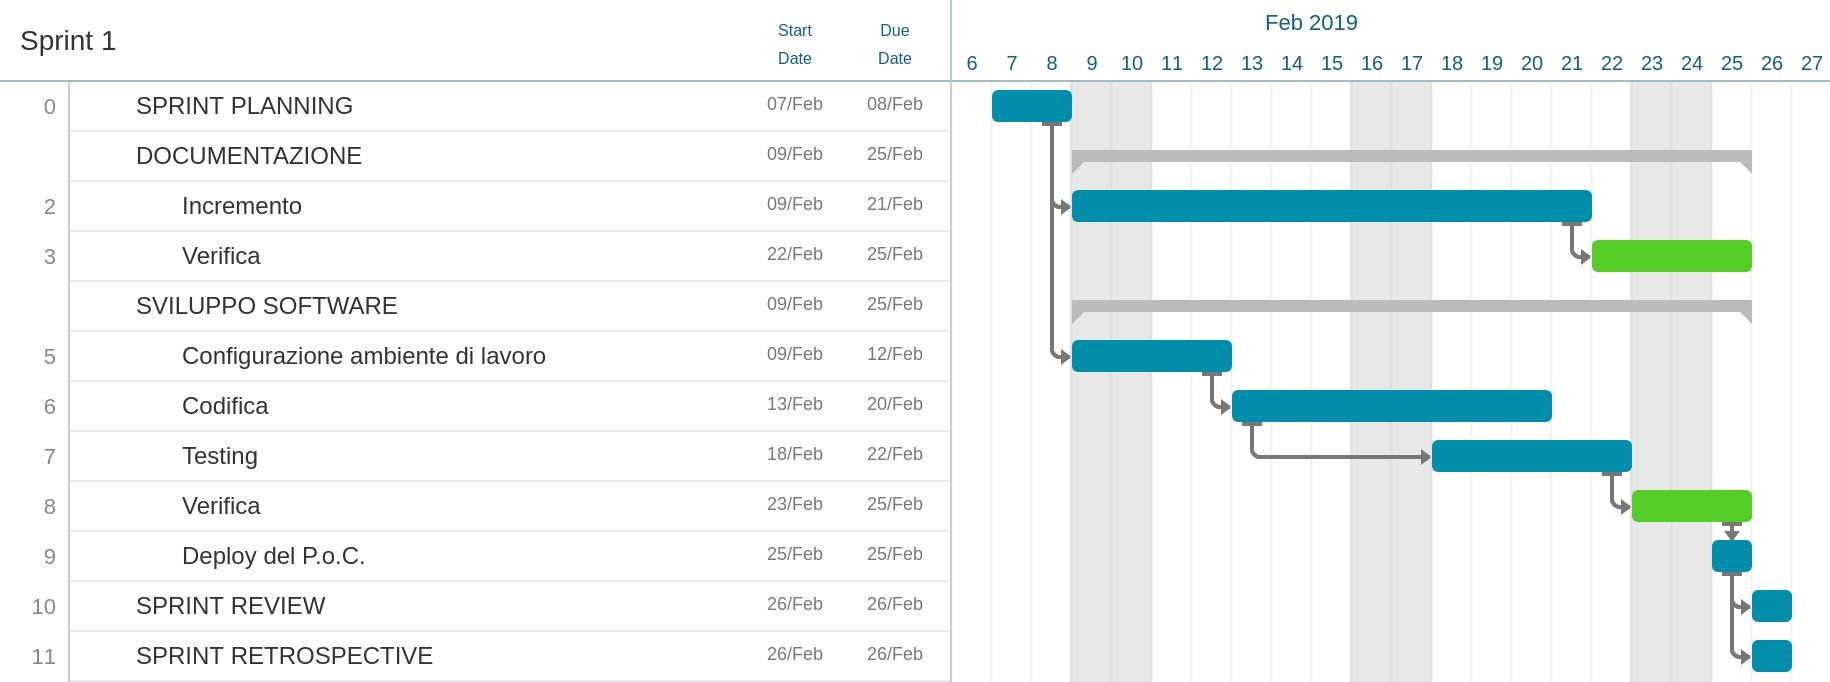
\includegraphics[width=15cm,keepaspectratio]{../includes/pics/grafici/Sprint_1.jpeg}
	\caption{\label{fig:gantt-sprint1}diagramma di Gantt del primo Sprint}
\end{figure}

\clearpage
\subsubsection{Sprint 2}
Il secondo sprint inizia il 27-02-2019 e finisce il 19-03-2019. Nel corso di questa iterazione, si effettua la consegna del P.o.C. realizzato nello sprint precedente e si riceve un primo feedback sul prodotto.
Nel dettaglio, le attività da svolgere in questo ciclo sono:
	\begin{itemize}
		\item \textbf{Sprint Planning}: si tratta di una riunione ad inizio sprint, nella quale il team si accorda sugli obiettivi da raggiungere entro fine sprint. Inoltre vengono identificati i requisiti necessari al completamento delle singole attività;
		\item \textbf{Discussione Agile}: consiste in una videoconferenza con il proponente, nella quale il team \emph{duckware} illustrerà il P.o.C. realizzato durante lo sprint precedente, le funzionalità implementate e da implementare, nonchè le tecnologie utilizzate durante lo sviluppo. Si tratta di un'attività critica in quanto è richiesto il suo superamento per poter avanzare alla fase di progetto successiva;
		\item \textbf{Meeting Post-Discussione}: in seguito alla \emph{Discussione Agile}, i membri di \emph{duckware} dovranno analizzare il feedback ricevuto durante la presentazione del P.o.C. ed aggiornare il Backlog in modo da rientrare nelle richieste degli stakeholder;
		\item \textbf{Product Baseline}: in questa attività si prevede la costruzione della \markg{baseline} architetturale del prodotto tramite diagrammi delle classi e di sequenza, va inoltre dimostrata la coerenza con quanto mostrato durante la \emph{Technology Baseline};
		\item \textbf{Sviluppo Software}: questa attività è preclusa dal soddisfacimento dell'attività precedente, in quanto consiste nel tradurre in codice quanto stabilito nella \emph{Product Baseline}. Essa consiste in un periodo di codifica con relativo testing, e prevede la verifica sia statica che dinamica di quanto prodotto.
		\item \textbf{Incremento e Verifica}: in questa attività vengono eseguite delle procedure di adeguamento al feedback, incremento e verifica sui documenti e sulla Technology Baseline, seguendo le indicazioni risultanti dalla Revisione dei Progettazione. Come detto in \addref{sec:technology_baseline}, la parola "incremento" è da intendersi come aggiunta di valore al prodotto in seguito ad una iterazione e non come un approccio propriamente incrementale;
		\item \textbf{Lettera di presentazione}: in questa attività si prevede la stesura della Lettera di presentazione per la \emph{Revisione di Progettazione};
		\item \textbf{Consegna[RP]}:questa attività indica il termine ultimo per la consegna dei documenti riguardanti la \emph{Revisione di Progettazione}. Vengono consegnati quindi i documenti richiesti, aggiornati allo sprint precedente. Non è possibile effettuare la consegna, e di conseguenza partecipare alla revisione, se la \emph{Discussione Agile} non soddisfa i proponenti;
		\item \textbf{Sprint Review}: si tratta di un meeting di fine sprint ed ha lo scopo di verificare quali funzionalità sono state implementate durante il corrente sprint;
		\item \textbf{Sprint Retrospective}: segue lo \emph{Sprint Review} ed è un incontro in cui il team di sviluppo discute su quanto è stato fatto durante lo sprint, sulle difficoltà avute durante lo sviluppo e sulle migliorie che si potrebbero apportare in futuri sprint.  
	\end{itemize}
\begin{figure}[htbp]
	\centering
	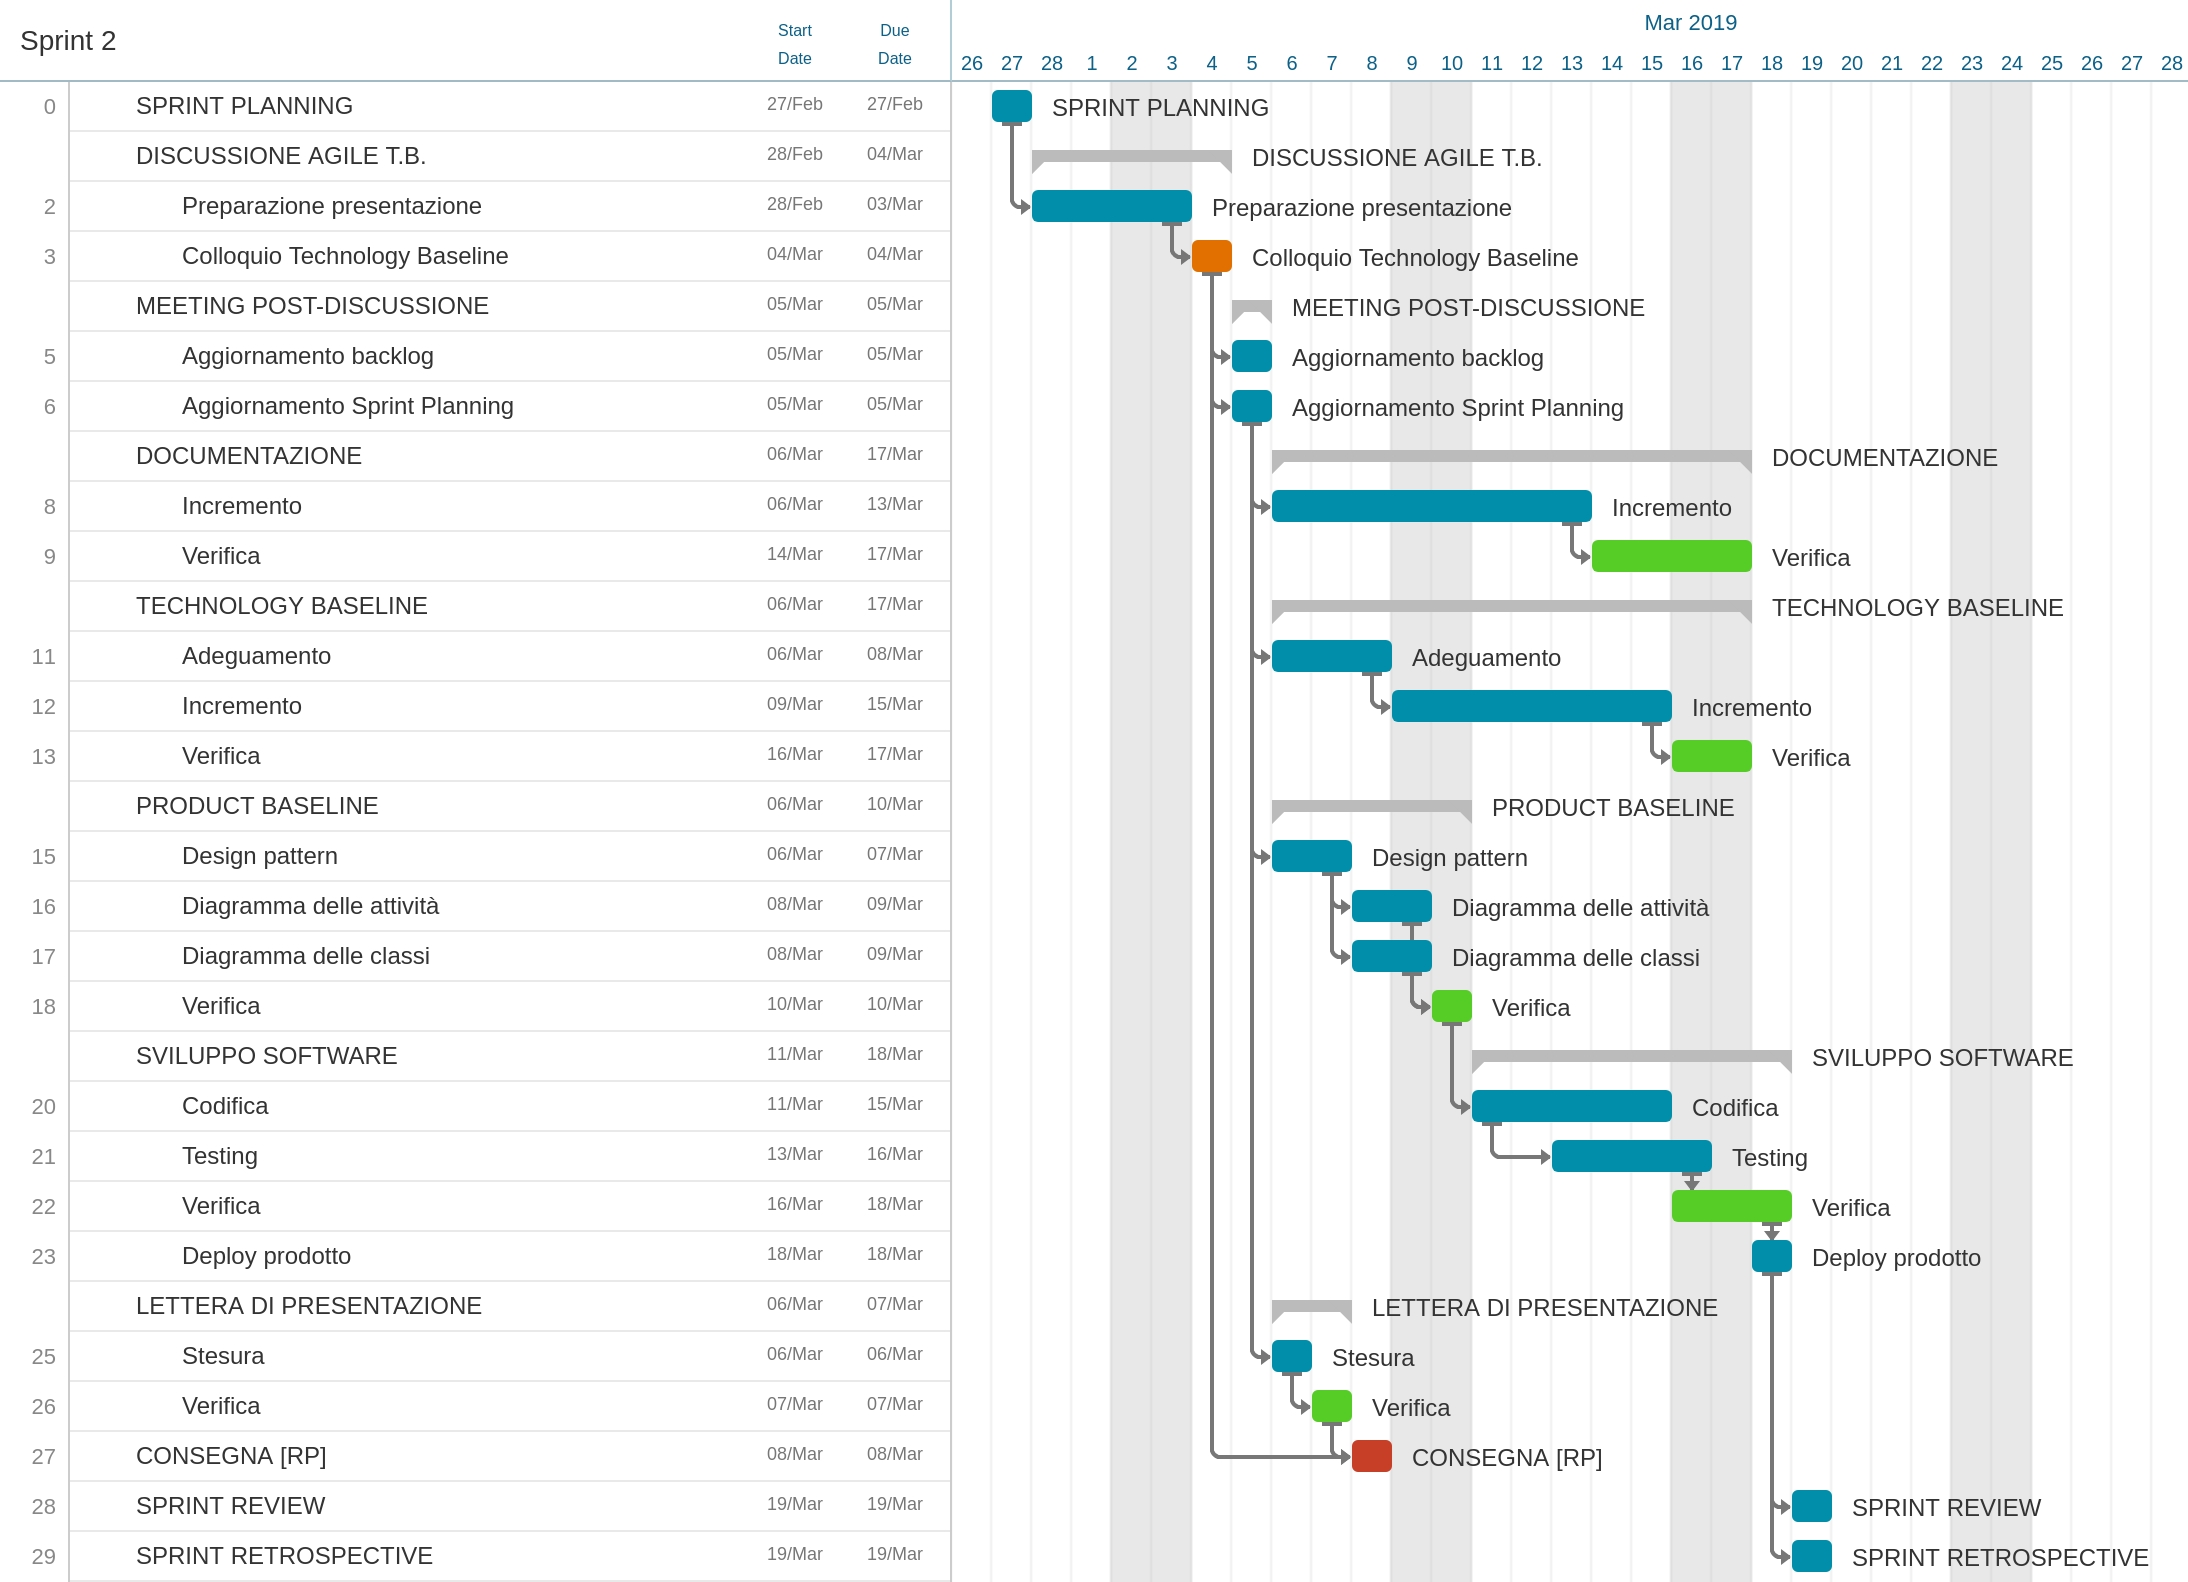
\includegraphics[width=15cm,keepaspectratio]{../includes/pics/grafici/Sprint_2.jpeg}
	\caption{\label{fig:gantt-sprint2}diagramma di Gantt del secondo Sprint}
\end{figure}

\clearpage
\subsubsection{Sprint 3}
Il terzo sprint dura dal 20-03-2019 al 09-04-2019. Nel corso di questo sprint, il team \emph{duckware} deve continuare a sviluppare il prodotto seguendo l'architettura descritta nella \emph{Product Baseline}. Inoltre, si iniziano a redigere il manuale sviluppatore e il manuale utente.
Le attività pianificate per questa iterazione sono:
	\begin{itemize}
		\item \textbf{Discussione Feedback}: come nelle fasi precedenti, questa attività consiste nella discussione e analisi degli esiti e delle eventuali problematiche emerse dalla consegna della \emph{Revisione di Progettazione};	
		\item \textbf{Sprint Planning}: si tratta di una riunione ad inizio sprint, nella quale il team si accorda sugli obiettivi da raggiungere entro fine sprint. Inoltre vengono identificati i requisiti necessari al completamento delle singole attività;
		\item \textbf{Incremento e Verifica}: in questa attività, ad inizio periodo, vengono eseguite delle procedure di incremento e verifica sui documenti \emph{Norme di Progetto, Piano di Progetto, Piano di Qualifica e Product Baseline} seguendo le indicazioni risultanti dalla Revisione di Progettazione;
		\item \textbf{Stesura dei Manuali}: in questa attività si prevede la realizzazione di un \emph{Manuale Utente} contenente indicazioni e direttive sulla configurazione e l'utilizzo del prodotto a livello utente, e di un \emph{Manuale Sviluppatore} in cui sono illustrati i design pattern implementati, i diagrammi delle classi e i diagrammi delle attività, così da rendere il codice più facilmente mantenibile;
		\item \textbf{Sprint Review}: si tratta di un meeting di fine sprint ed ha lo scopo di verificare quali funzionalità sono state implementate durante il corrente sprint;
		\item \textbf{Sprint Retrospective}: segue lo \emph{Sprint Review} ed è un incontro in cui il team di sviluppo discute su quanto è stato fatto durante lo sprint, sulle difficoltà avute durante lo sviluppo e sulle migliorie che si potrebbero apportare in futuri sprint;
		\item \textbf{Discussione Agile}: a differenza del colloquio precedente, in questa videoconferenza si discute la \emph{Product Baseline}, quindi l'utilizzo dei corretti design pattern e il corretto tracciamento dei diagrammi delle classi e delle attività. L'approvazione in questa sede, permette al team di consegnare la documentazione necessaria per l'entrata in \emph{Revisione di Accettazione}.
	\end{itemize}
\begin{figure}[htbp]
	\centering
	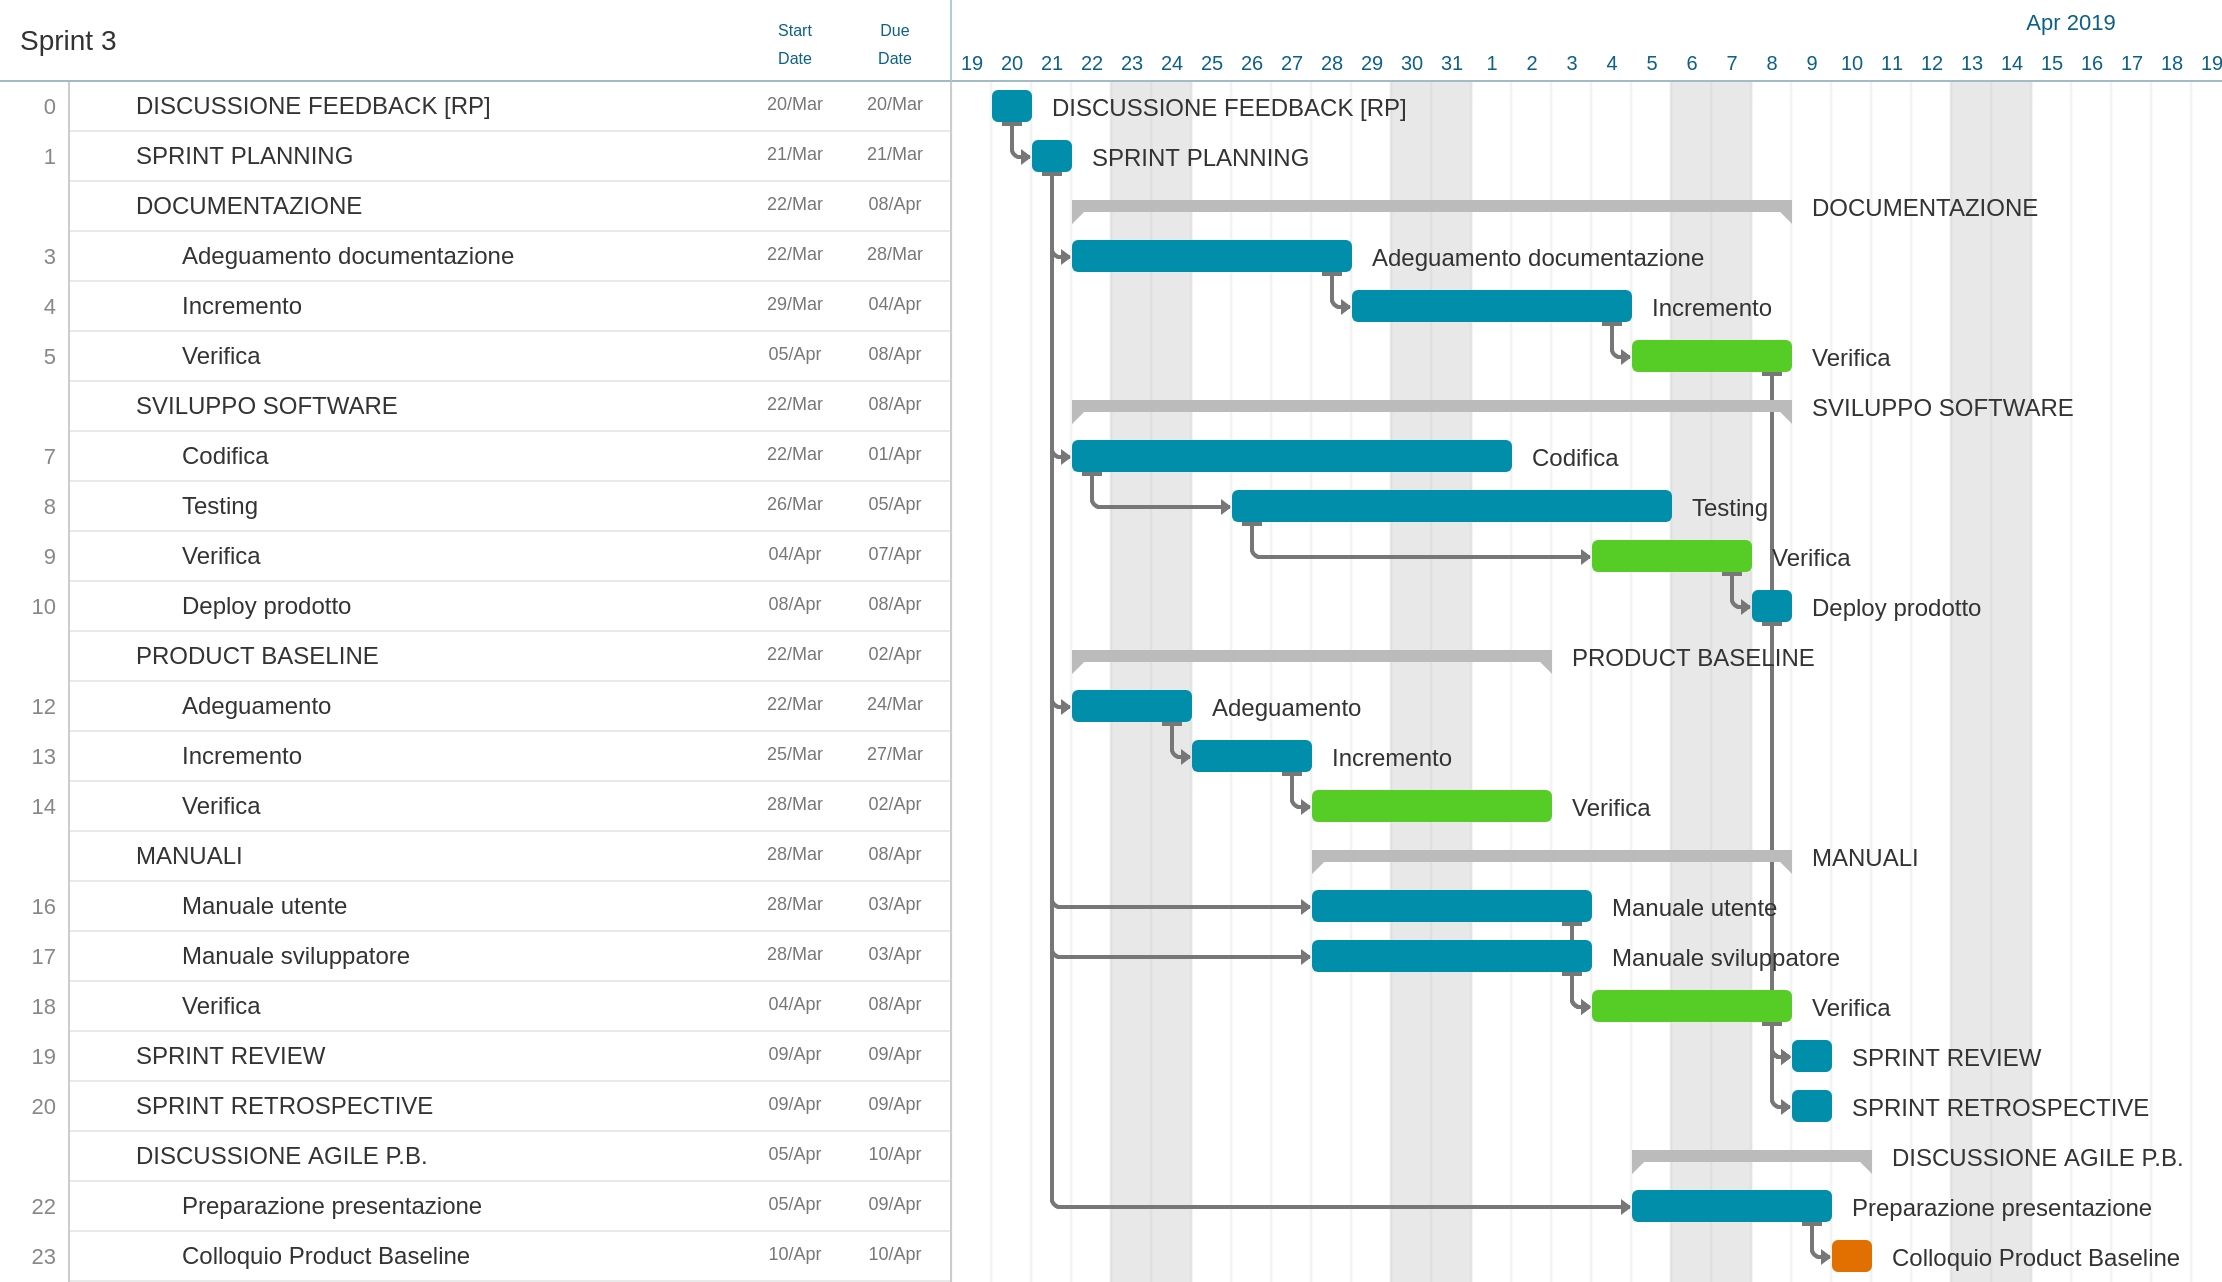
\includegraphics[width=15cm,keepaspectratio]{../includes/pics/grafici/Sprint_3.jpeg}
	\caption{\label{fig:gantt-sprint3}diagramma di Gantt del terzo Sprint}
\end{figure}

\clearpage
\subsubsection{Sprint 4}
La quarta iterazione inizia con la consegna della documentazione necessaria per l'entrata in \emph{Revisione di Accettazione}, il 12-04-2019, e termina il 01-05-2019. Questo ciclo si focalizza sull'implementazione dei requisiti opzionali, sulla verifica statica e dinamica del codice del prodotto e sulla stesura dei manuali.
Le task pianificate per questo sprint sono le seguenti:
	\begin{itemize}
		\item \textbf{Sprint Planning}: si tratta di una riunione ad inizio sprint, nella quale il team si accorda sugli obiettivi da raggiungere entro fine sprint. Inoltre vengono identificati i requisiti necessari al completamento delle singole attività;
		\item \textbf{Incremento e Verifica}: in questa attività, ad inizio sprint, vengono eseguite delle procedure di incremento e verifica sui documenti \emph{Norme di Progetto, Piano di Progetto, Piano di Qualifica, Product Baseline, Manuale Utente e Manuale Sviluppatore} seguendo le indicazioni risultanti dalla Revisione di Qualifica;
		\item \textbf{Sviluppo Software}: implementazione delle funzionalità opzionali e ottimizzazione del codice. Vengono eseguite attività di Analisi statica e dinamica del codice, così da assicurare consistenza con quanto scritto nel \emph{Piano di Qualifica} e nelle \emph{Norme di Progetto};
		\item \textbf{Sprint Review}: si tratta di un meeting di fine sprint ed ha lo scopo di verificare quali funzionalità sono state implementate durante il corrente sprint;
		\item \textbf{Sprint Retrospective}: segue lo \emph{Sprint Review} ed è un incontro in cui il team di sviluppo discute su quanto è stato fatto durante lo sprint, sulle difficoltà avute durante lo sviluppo e sulle migliorie che si potrebbero apportare in futuri sprint.
	\end{itemize}
\begin{figure}[htbp]
	\centering
	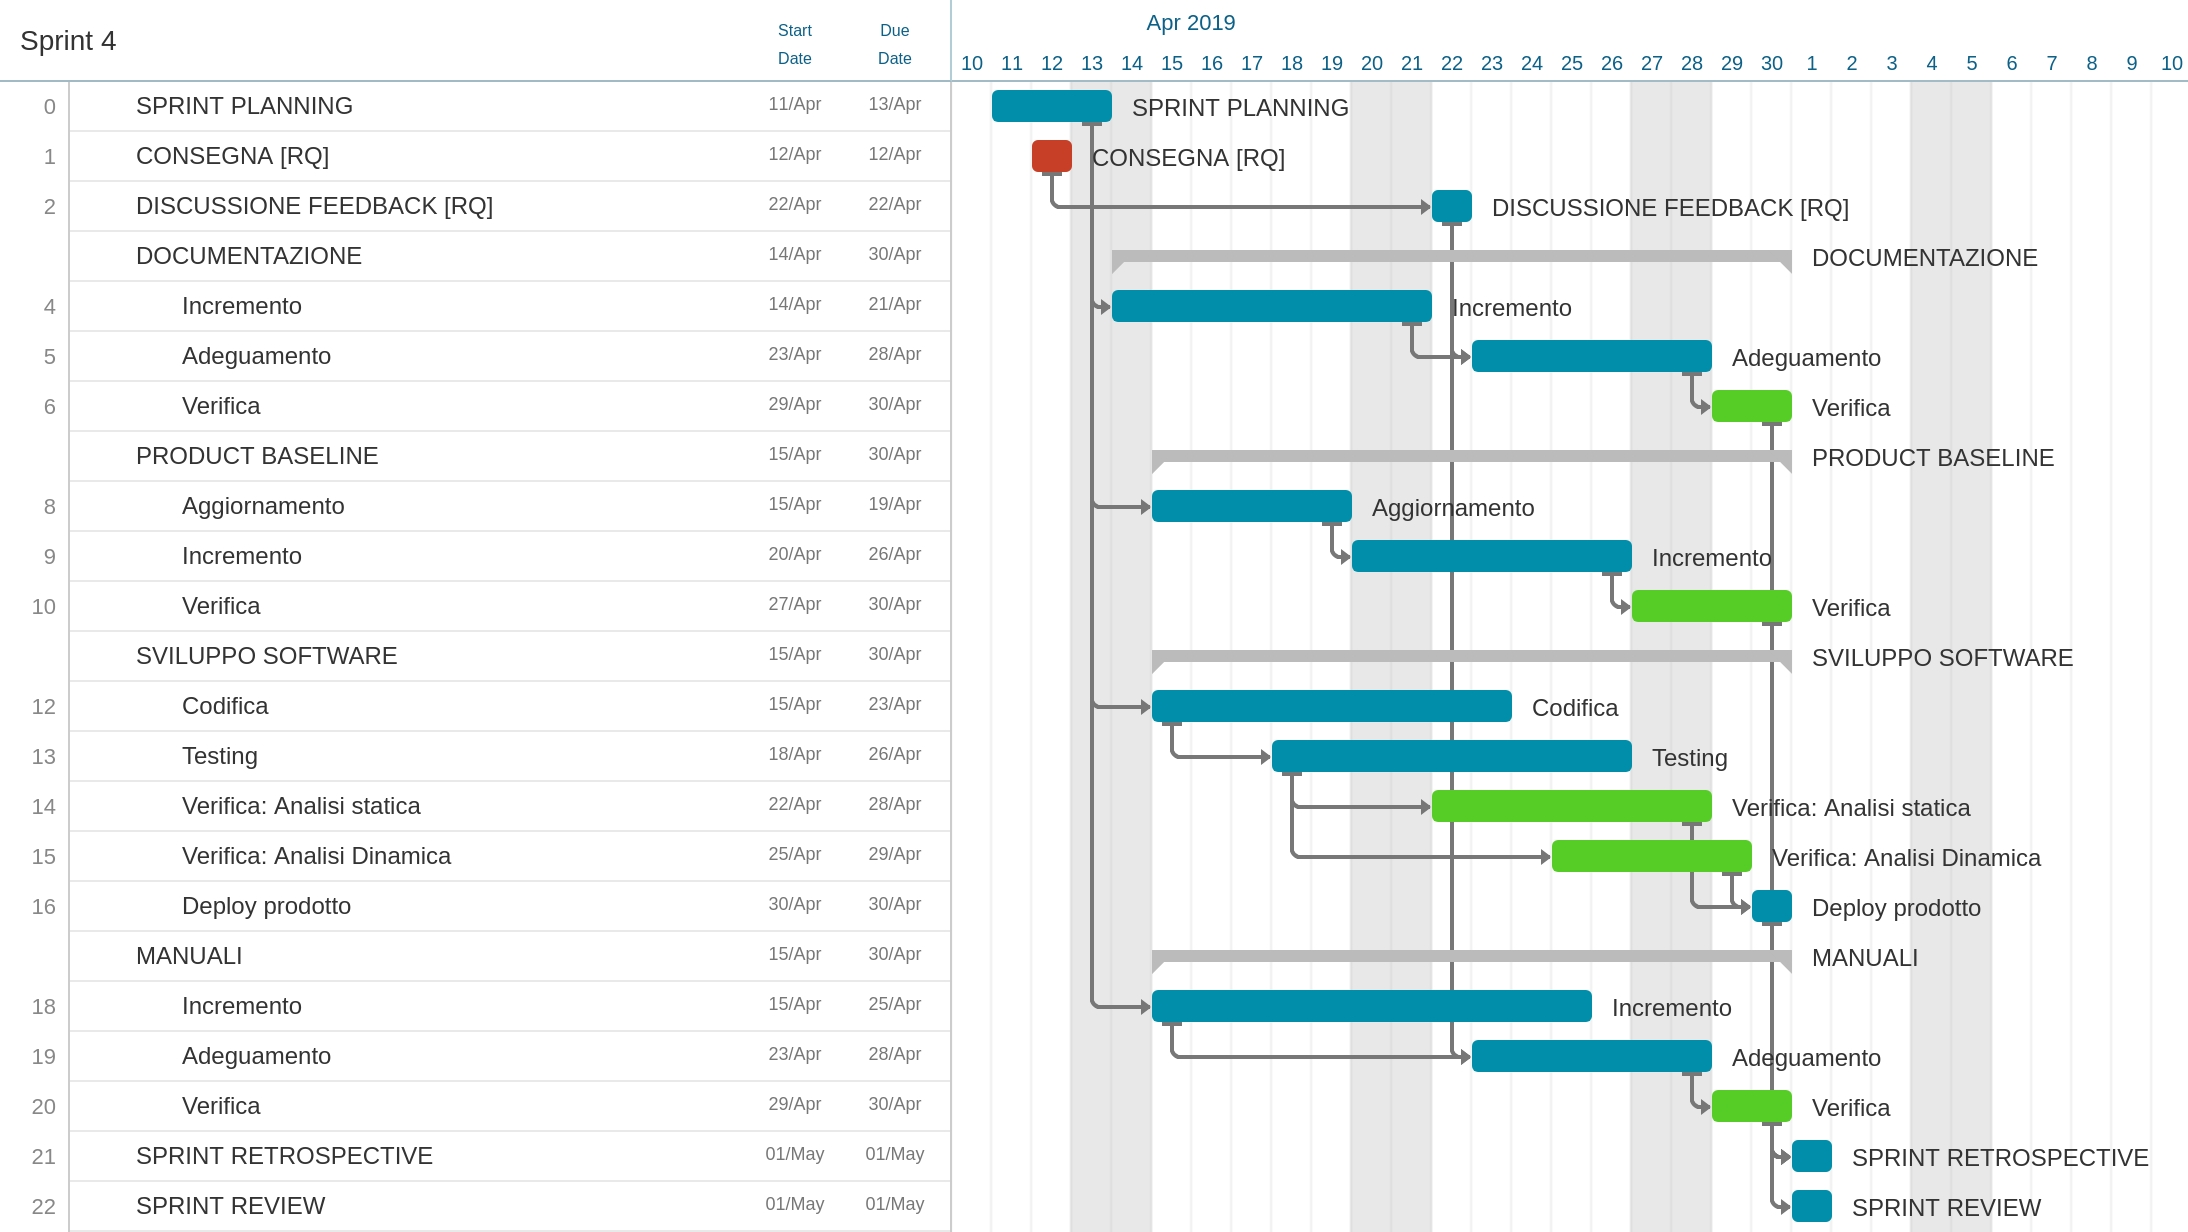
\includegraphics[width=15cm,keepaspectratio]{../includes/pics/grafici/Sprint_4.jpeg}
	\caption{\label{fig:gantt-sprint4}diagramma di Gantt del quarto Sprint}
\end{figure}

\clearpage
\subsubsection{Sprint 5}
Il quinto Sprint comincia il 02-05-2019 e termina con la presentazione del prodotto finito, ovvero il 17-05-2019. Questa iterazione risulta essere leggermente più corta rispetto alle precedenti, in quanto anche meno onerosa per i membri del gruppo. Essa infatti si focalizzerà nel perfezionamento dei dettagli del prodotto e sulla validazione di tutti i requisiti, pertanto, le attività pianificate risultano essere:
	\begin{itemize}
		\item \textbf{Sprint Planning}: si tratta di una riunione ad inizio sprint, nella quale il team si accorda sugli obiettivi da raggiungere entro fine sprint. Inoltre vengono identificati i requisiti necessari al completamento delle singole attività;
		\item \textbf{Incremento e Verifica}: in questa attività, ad inizio iterazione, vengono eseguite delle procedure di incremento e verifica sui documenti \emph{Norme di Progetto, Piano di Progetto, Piano di Qualifica, Product Baseline, Manuale Utente e Manuale Sviluppatore} seguendo i feedback ricevuti durante lo sprint precedente;
		\item \textbf{Sviluppo Software}: in questa attività è prevista l'esecuzione di test e miglioramenti dell'applicativo prodotto per garantire il soddisfacimento dei vincoli qualitativi;
		\item \textbf{Consegna [RA]}: durante questa task verranno consegnati tutti i documenti attinenti lo sviluppo del prodotto, e il prodotto stesso tramite supporto fisico.
	\end{itemize}
\begin{figure}[htbp]
	\centering
	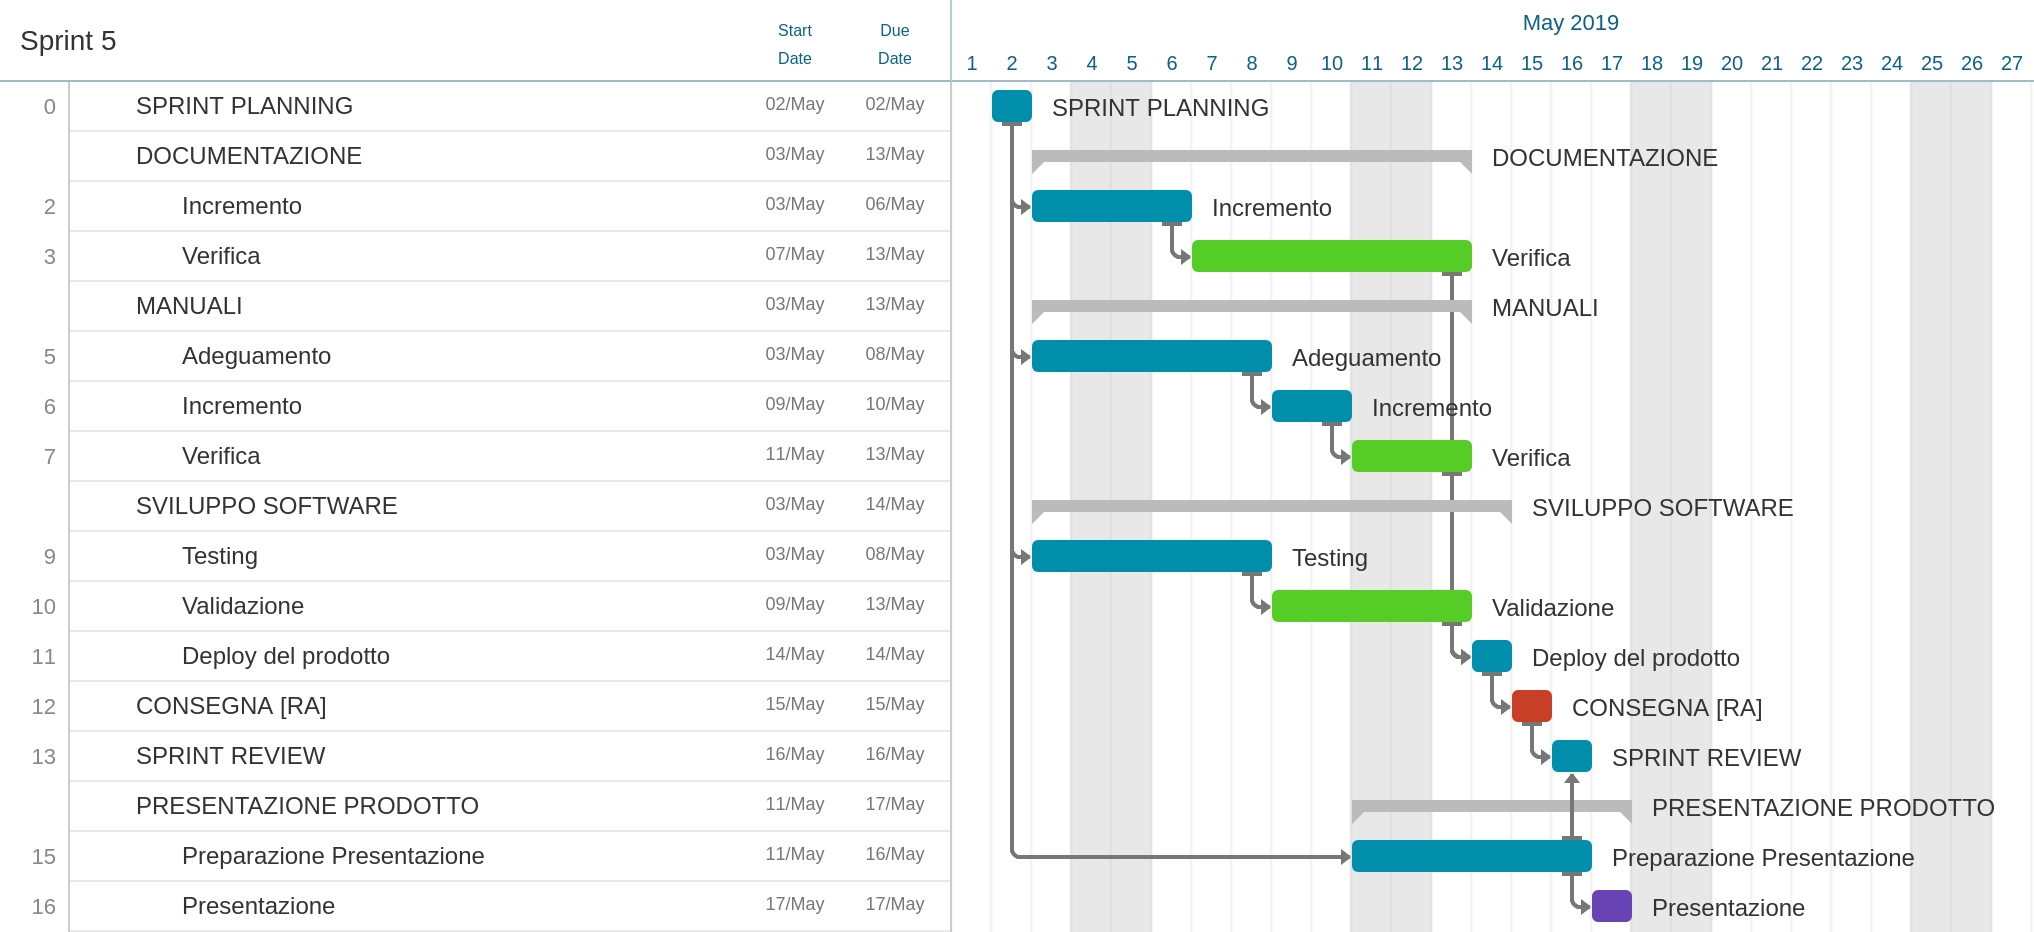
\includegraphics[width=15cm,keepaspectratio]{../includes/pics/grafici/Sprint_5.jpeg}
	\caption{\label{fig:gantt-sprint5}diagramma di Gantt del quinto Sprint}
\end{figure}




